Electrolyte-gated field-effect transistors (EG-FETs) are a subgoup of field-effect transistors: they share the same design and concept, with the gate electrode controlling the current flowing between source and drain, through the application of a voltage on a dielectric material, that causes the formation of an electric field. While they share electrode design, they differ in the choice of dielectric: EG-FETs, as a matter of fact, employ high-capacitance electrolytes as dielectrics, which enable more efficient coupling between the gate and the channel; this phenomenon makes it possible to induce a strong electric field effect on the channel, even in the presence of small changes in gate voltage \citet{kimElectrolyteGated2013, wangElectrolytic2016}. The working mechanism that will be explained in detail in the paragraph \nameref{par:mechanismEGFET}.

In addition to their enhanced sensitivity, EG-FETs address some of the limitations of other devices by enabling the detection of biomolecules in their native aqueous environments, an essential feature for biological sensing applications \citep{wangElectrolytic2016}.

\paragraph{Configurations of EG-FETs}

\begin{figure}[ht]
    \centering
    \subfloat[MIPs]{%
        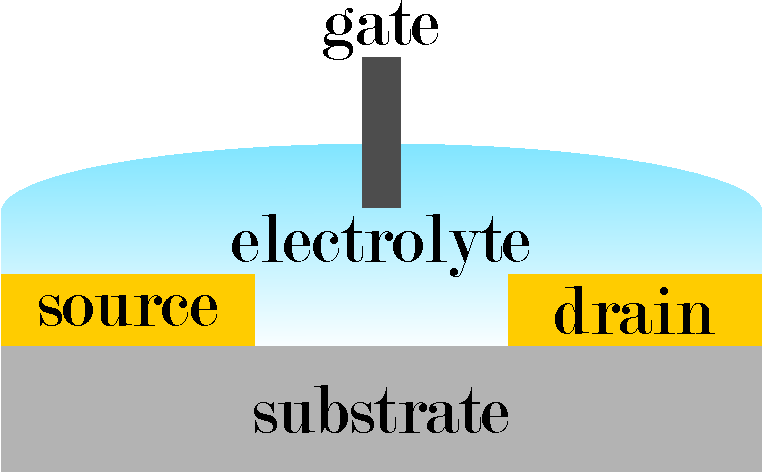
\includegraphics[width=0.3\textwidth]{figures/chapter1/egfet/Fig5_topGateEGFET.pdf}
        \label{fig:topGate}
    }
    \hspace{0.05\textwidth}
    \subfloat[Nano]{%
        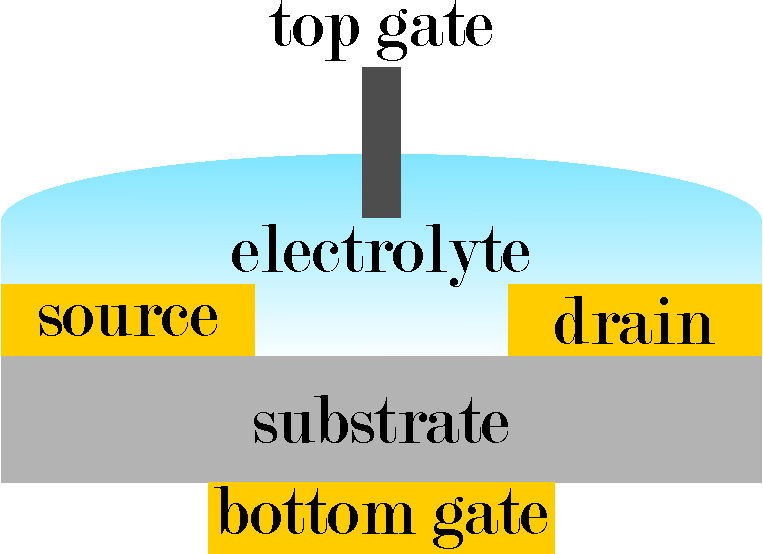
\includegraphics[width=0.3\textwidth]{figures/chapter1/egfet/Fig5_dualGateEGFET.pdf}
        \label{fig:dualGate}
    }
    \vskip 1em % Adds vertical space between rows
    \subfloat[Ab]{%
        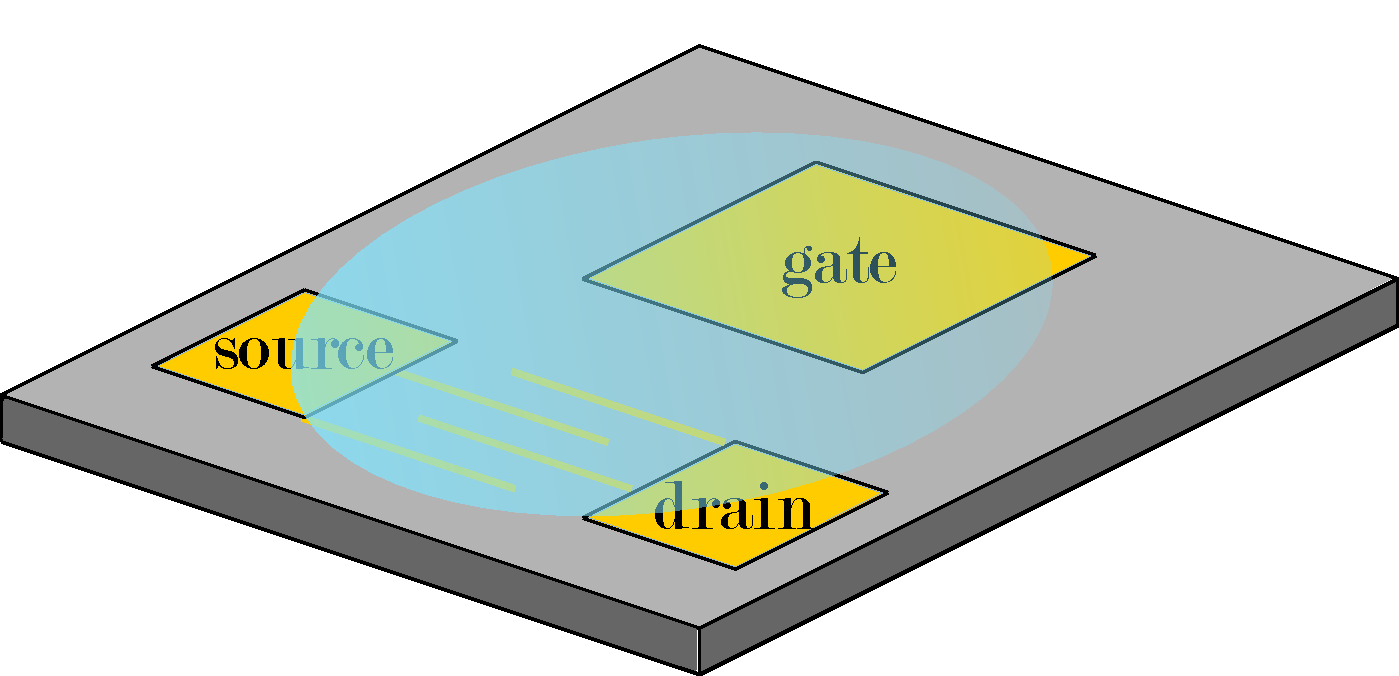
\includegraphics[width=0.3\textwidth]{figures/chapter1/egfet/Fig5_planarEGFET.pdf}
        \label{fig:planarGate}
    }
    \hspace{0.05\textwidth}
    %\hfill
    \subfloat[Enz]{%
        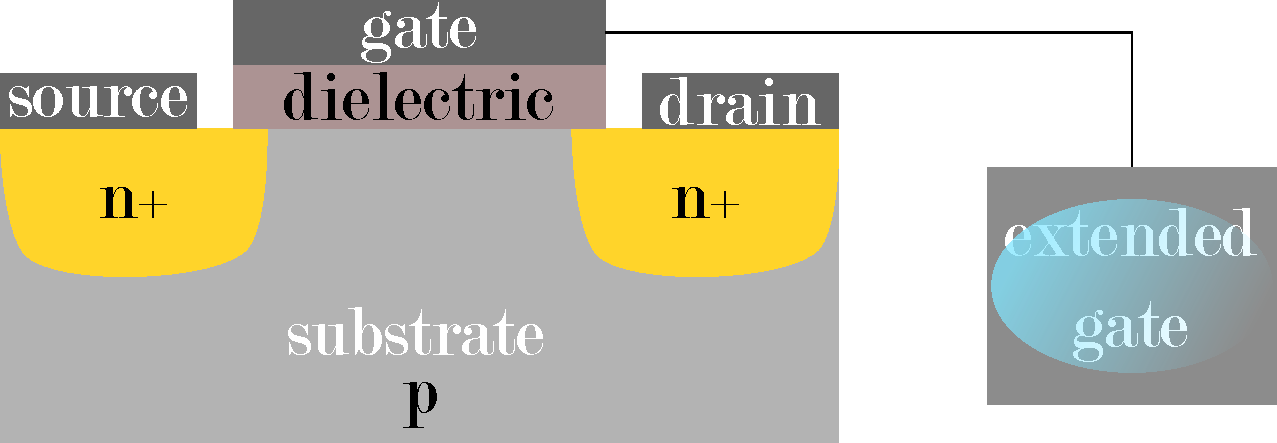
\includegraphics[width=0.3\textwidth]{figures/chapter1/egfet/Fig5_extendedEGFET.pdf}
        \label{fig:extendedGate}
    }
    \caption{Schematic representation of different electrolyte-gated field-effect transistor (EG-FET) configurations: (a) Top-gate, where the gate electrode and electrolyte are above the semiconductor channel; this is the most common configuration. (b) Dual-gate, incorporating both top and bottom gates allows to evaluate device parameters such as electric double layer capacitance. (c) Planar-gate, where the gate electrode is laterally positioned in the same plane as the semiconductor channel, granting ease of fabrication and providing a structure suitable for in-plane sensing applications, \eg{} integration in warable devices. (d) Extended-gate, in which the sensing gate electrode is physically separated from the transistor, enabling sensing in distinct environments, thus protecting the body of the device from the electrolyte.}
    \label{fig:egfetConfigs}
\end{figure}

Several configurations of EG-FETs exist, adapted to different fabrication methods and sensing needs \citep{shkodraElectrolytegated2021}.
The top gate-bottom contact design is the most common one, with the electrolyte on top of the channel, with source and drain electrodes beneath; a conventional reference electrode, typically made of \ce{Ag/AgCl} or \ce{Pt}, is positioned on top of the electrolyte, working as gate \citep{shkodraElectrolytegated2021}. The planar configuration positions the gate on the same plane as the channel, and source and drain electrodes; this feature is favoured for a simpler, faster fabrication \citep{joshiUnderstanding2018}. In extended gate EG-FETs, the gate is remotely placed and connected to the main FET; in this configuration, the body of the FET works as an amplifier, while the external gate is in contact with the electrolyte \citep{torricelliElectrolytegated2021}. This geometry prevents any damage that the electrolyte could make on the electrodes and semiconductor. Dual gate configurations, displaying a top- and a bottom-gate, exhibit higher stability, improved control, and robust long-term performance \citep{lagoRealtime2022}, while also allowing for precise measurements of the electric double layer capacitance \citep{cramerDouble2012, melzerCharacterization2014}.

\paragraph{Working Mechanism of EG-FETs}
\label{par:mechanismEGFET}

\begin{figure}[ht]
    \centering
    \subfloat[No voltage applied]{
        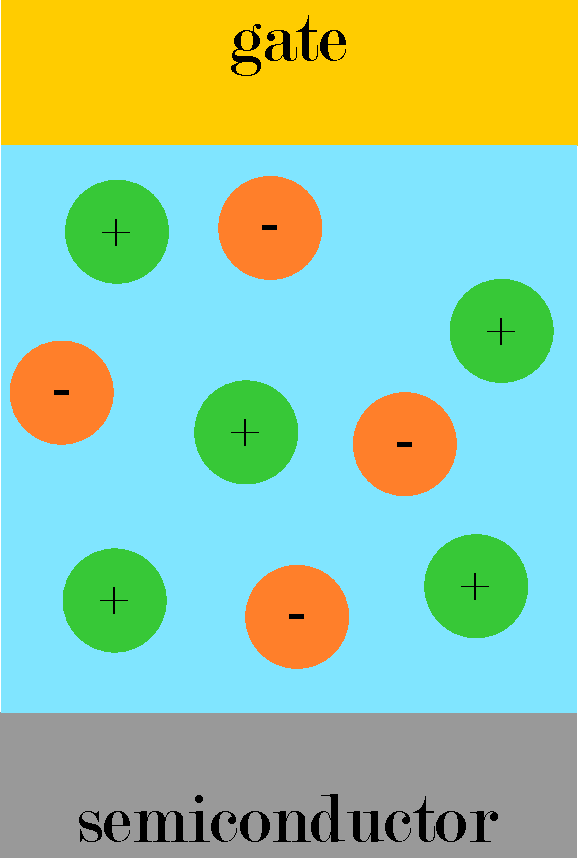
\includegraphics[height=4.6cm]{figures/chapter1/egfet/Fig6_EDL1.pdf}
        \label{fig:edl1}
    }
    \subfloat[\vgs{} applied]{
        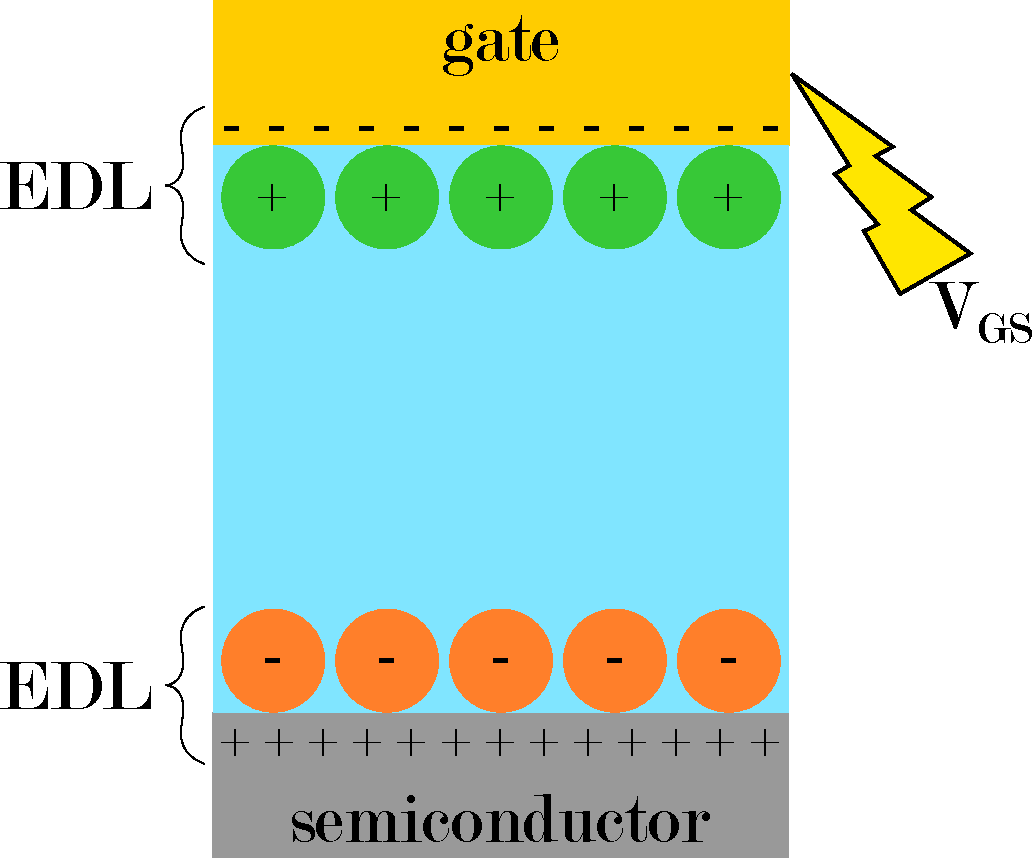
\includegraphics[height=4.6cm]{figures/chapter1/egfet/Fig6_EDL2.pdf}
        \label{fig:edl2}
        }
    \subfloat[\vgs{} and \vds{} applied]{
        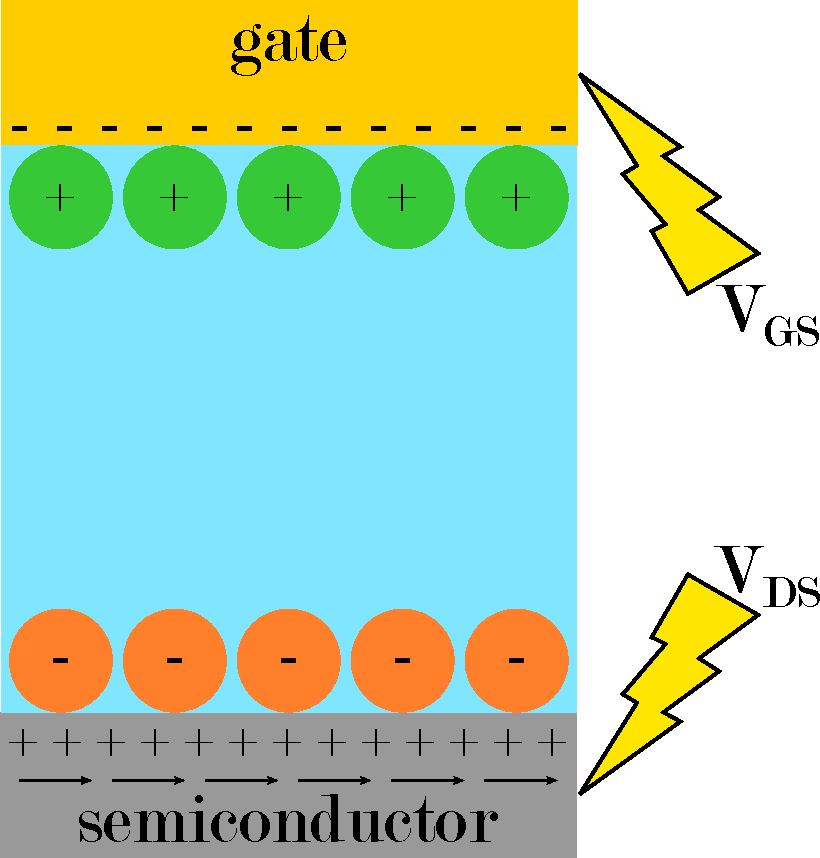
\includegraphics[height=4.6cm]{figures/chapter1/egfet/Fig6_EDL3.pdf}
        \label{fig:edl3}
        }
    \caption{Schematic illustration of the working mechanism of electrolyte-gated field-effect transistors (EG-FETs).
    (a) In the absence of an applied gate voltage, ions are freely dispersed in the electrolyte.
    (b) When a gate voltage is applied, the gate electrode becomes polarized, attracting counterions from the electrolyte and forming an electric double layer (EDL) at the gate-electrolyte interface. This induces an opposing EDL at the electrolyte-semiconductor interface, leading to charge carrier accumulation in the channel. The EDLs act as capacitor plates, replacing the conventional solid-state dielectric.
    (c) When a drain-source voltage is applied, charge carriers in the channel start flowing, enabling transistor operation.}
    \label{fig:EDL}
\end{figure}

EG-FETs do not have a solid-state dielectric, as \ce{SiO2} may be for MOSFETs; rather, their proper functioning depends on the formation of electric double layers (EDLs). Indeed, when a voltage is applied to the gate, the electrode surface becomes polarized, thus getting either positively or negatively charged, depending on the sign of the voltage input. The generated electric field, then causes counterions from the electrolyte to migrate in front of the electrode, effectively shielding the charged surface. The phenomenon herein described, visible in Figure \ref{fig:EDL}, happens in a parallel way at the semicondutor/electrolyte interface, with inverted charges. This charge accumulation modulates the conductivity of the semiconductor, but a minimum gate voltage, known as the threshold voltage (\vth{}), must be reached before a significant conductive channel forms and current flows between source and drain. The value of \vth{} depends on the properties of the semiconductor, the electrolyte, and the specific device configuration. This phenomenon takes the name of electric double layers: these parallel charges accumulations work as capacitor plates, indeed behaving as dielectric material, making EG-FETs highly effective in sensing applications \citep{kimElectrolyteGated2013, wangElectrolytic2016}. Behind each EDL, ion concentration decreases according to the Stern-modified Gouy-Chapman model \citep{oldhamGouy2008}. The region in which charges are screened is defined by the Debye length, explained more in detail in Section \ref{sec:simulations}.
Not only does this system preserve biological analytes in a near-native environment, but it also takes advantage of the thin EDL layers and the high relative permittivity of electrolytes to significantly amplify the signal;while a \ce{SiO2} dielctric has a relative permittivity of 3.9 and \ce{Al2O3} has a relative permittivity of 9.5, phosphate buffer saline (PBS) has a relative permittivity of 79, leading to capacitances 100 to 1000 times higher, in the order of \SI{}{\uF\per\cm\squared} \citep{shkodraElectrolytegated2021,velickyElectrolyte2021}. This high capacitance amplifies field effects, enhancing the device's sensitivity and signal strength \citep{shkodraElectrolytegated2021}. As a result, a small gate bias, often below \SI{1}{V}, can be applied to achieve measurable results while avoiding electrolysis of the aqueous electrolyte, which occurs at \SI{1.23}{V} \citep{suoWaterinsalt2015}.

\paragraph{EG-FET-based (bio)sensors}
EG-FETs have been successfully employed as trasnducers for (bio)sensors for various applications, including environmental monitoring, health surveillance, and food safety, showcasing their versatility.

In environmental monitoring, EG-FETs detect dangerous contaminants such as mercury, ammonia, and pesticides. \citet{knopfmacherHighly2014} developed a mercury sensor using a DNA probe conjugated to gold nanoparticles, later improved by \citet{alqahtaniBridged2023} with an ion-exchange resin. \citet{singhFabrication2021} designed an EG-FET with \ce{CuO} nanowires for ammonia detection, while \citet{sasipongpanaExtended2017} used AChE-functionalized EG-FETs to quantify pesticide levels by monitoring enzyme inhibition. More recently, \citet{elliElectrolyteGated2024} developed an EG-CNTFET for detecting polystyrene nanoparticles in seawater, addressing microplastic pollution. Additional applications are reviewed by \citet{pullanoEGFETBased2018} and \citet{elliFieldEffect2022}.

EG-FETs have also advanced health monitoring, especially through biomarker detection. \citet{iskierkoExtendedgate2015} developed an EG-FET functionalized with molecularly imprinted polymers for inosine, a biomarker of renal dysfunction and diabetic nephropathy. \citet{macchiaSelective2019} fabricated an ultra-sensitive EG-FET to detect single molecules of C-reactive protein (CRP), while \citet{purwidyantriColloidal2018} created a DNA-functionalized EG-FET to detect \textit{Staphylococcus aureus}. In non-invasive monitoring, EG-FET sensors track ammonium levels in sweat, an indicator of muscle fatigue \citep{chenInvolvement2020, petrelliFlexible2022, petrelliNovel2022, petrelliMethod2023}.

In food safety, EG-FETs detect foodborne pathogens, toxins, and allergens. \citet{zaidanRapid2024} developed an EG-FET with a boron nitride-reduced graphene oxide (BN-rGO) gel functionalized with anti-\textit{E. coli} antibodies, while \citet{xiangInkjetPrinted2016} created a graphene-FET for norovirus. Mycotoxins and biogenic amines, including histamine and spermidine, have been targeted using EG-FET strategies \citep{ahDetection2012, minamiExtendedgate2015, shkodraFlexible2021, shkodraPolymeric2024}. Additionally, EG-FETs aid allergen detection, as seen in \citet{kimUltrasensitive2022} for peanut allergens. More comprehensive reviews on foodborne hazard sensors can be found in \citet{bobrinetskiyAdvances2021, kourtiOptical2023}.
